
\subsubsection{18.10.14}

\begin{enumerate}
	\item Время начала и окончания собрания:
	16:30 - 21:40
	\item Цели собрания:
	\begin{enumerate}
	  \item Создать окончательную версию захвата.
	  
	  \item Изменить программу управления захватом на более удобную.
	  
    \end{enumerate}
    
	\item Проделанная работа:
	\begin{enumerate}
	  \item Поперечная балка передвинута дальше от оси вращения захвата.
      
      \item Стяжки размещены на оси в 4 ряда через каждые 90° и закреплены термоклеем.
      
      \begin{figure}[H]
      	\begin{minipage}[h]{0.47\linewidth}
      		\center{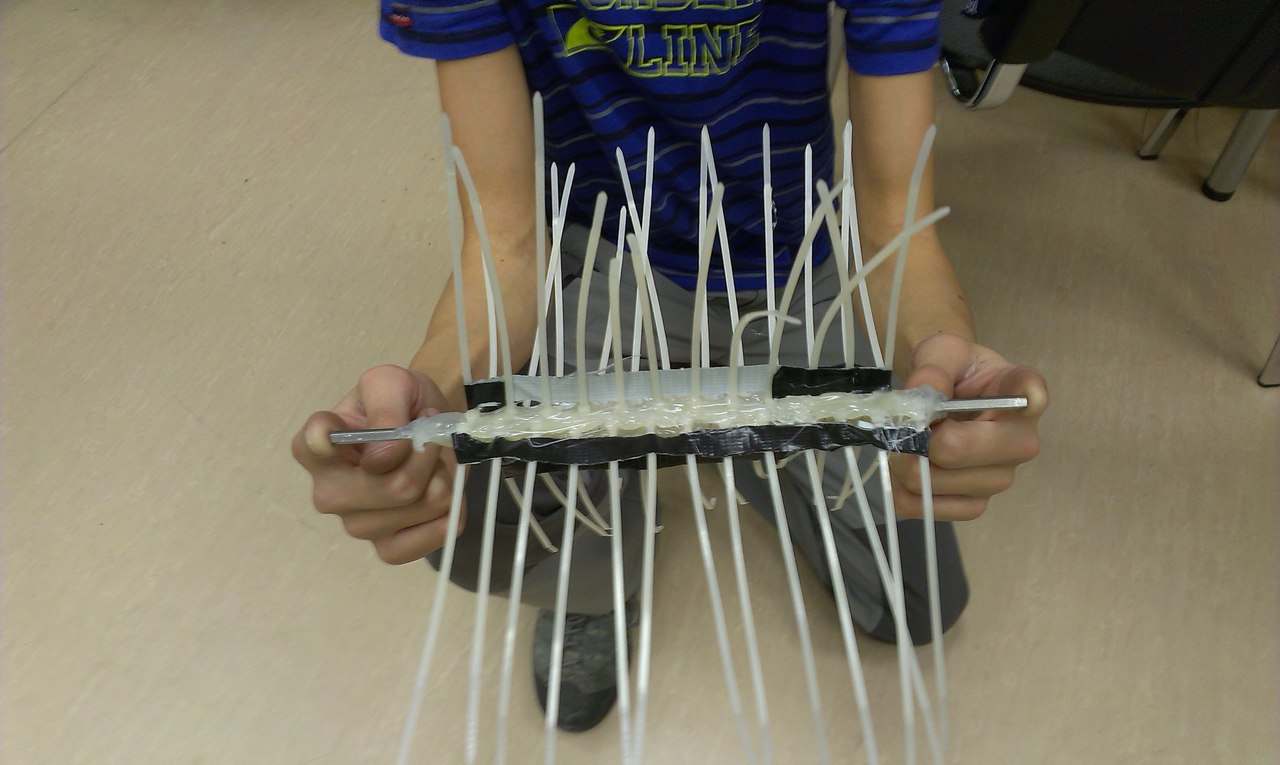
\includegraphics[scale=0.2]{days/images/Z0JBRRFYD8o}}
      		\caption{Щетка захвата}
      	\end{minipage}
      	\hfill
      	\begin{minipage}[h]{0.47\linewidth}
      		\center{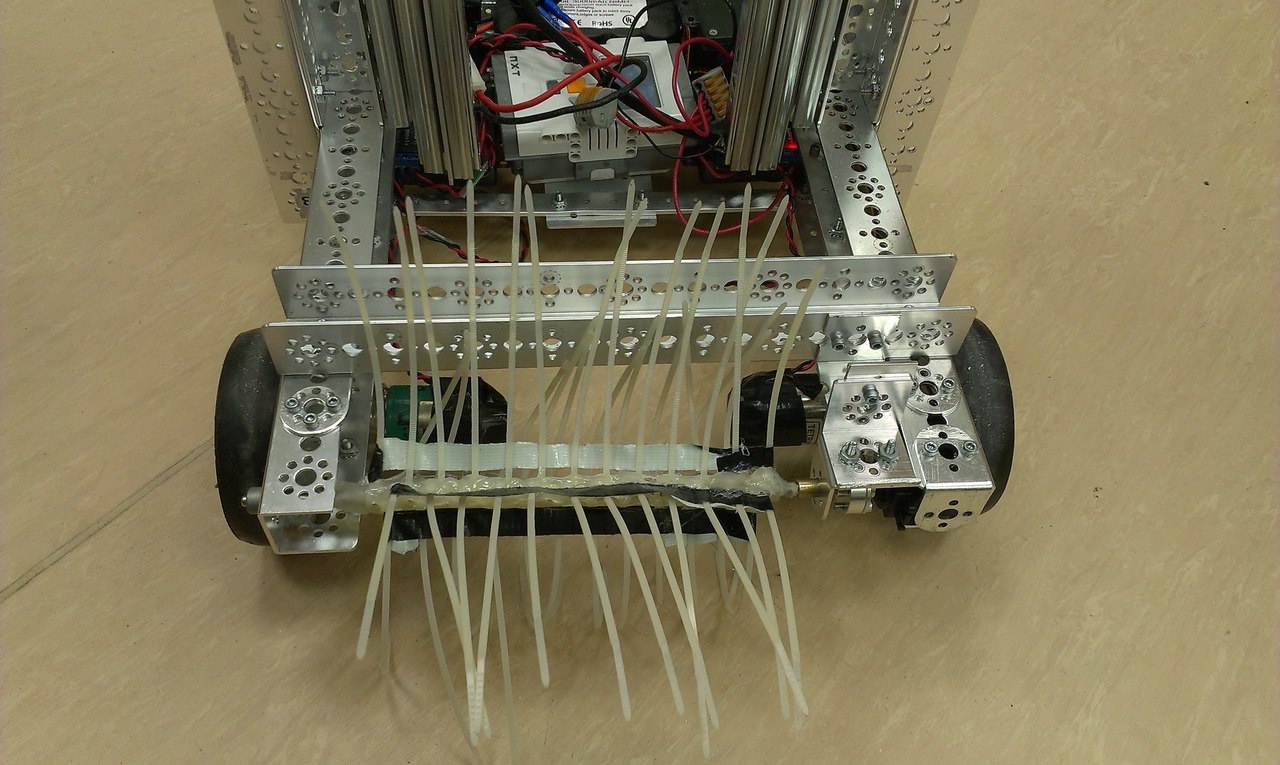
\includegraphics[scale=0.2]{days/images/NVWKh0xoKQM}}
      		\caption{Окончательная версия механизма захвата мячей}
      	\end{minipage}
      \end{figure}
      
      \item Программа управления захватом заменена. Теперь сервопривод меняет свое состояние (стоит или работает) по нажатию кнопки. Это позволяет оператору не отвлекаться на поддержание захвата в работающем состоянии.
      
      \item Были проведены полноценные испытания захвата с двумя мячами из набора NXT диаметром 5 см. Испытания прошли успешно, робот был способен захватывать мячи, расположенные как на открытом пространстве, так и возле стены. Некоторое неудобство доставлял тот факт, что щетка захвата расположена не вдоль всей передней кромки робота, а только посередине, поэтому для захвата мяча требовалось к нему прицеливаться. Впоследствии мы планируем устранить этот недостаток, установив по бокам от захвата балки, расположенные в виде воронки (далее они будут называться откосами), что позволит шарикам самостоятельно закатываться в область действия захвата.
      
      \item При программировании сервопривода свободного вращения выяснилось, что при постановке его на нейтраль он стремится удерживать угол, из-за чего начинает дребезжать. Этот баг необходимо исправить.
      
      \item Во время испытаний было замечено, что робот почти перестал дребезжать при поворотах корпуса. Как оказалось, это произошло по причине того, что большая часть его массы была сконцентрирована в задней части и передние колеса свободно проскальзывали. Это не было сделано специально, но тем не менее это усовершенствование дало в целом положительный результат.
      
      \item Помимо изначальных задач нами был сконструирован и закреплен на роботе механизм для опрокидывания ковша.
      
      \begin{figure}[H]
      	\begin{minipage}[h]{1\linewidth}
      		\center{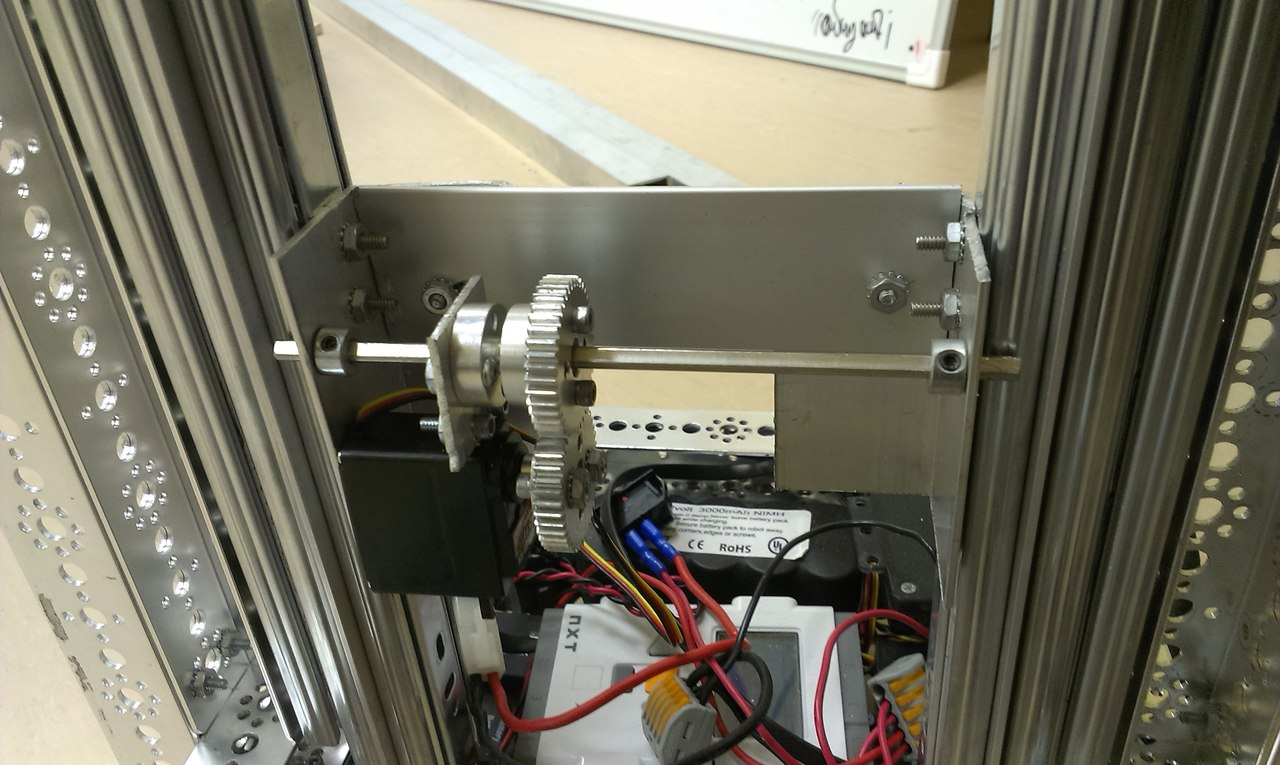
\includegraphics[scale=0.2]{days/images/LVPCEoPaC6M}}
      		\caption{Механизм для опрокидывания ковша}
      	\end{minipage}
      \end{figure}
      
    \end{enumerate}
    
	\item Итоги собрания: 
	\begin{enumerate}
	  \item Завершена работа над механизмом захвата.
	  
      \item Создана удобная программа для управления захватом.
      
    \end{enumerate}
    
	\item Задачи для последующих собраний:
	\begin{enumerate}
	  \item Исправить баг с сервоприводом свободного вращения.
	  
	  \item Укрепить ограничители хода мебельных реек.
	  
	  \item Установить балки помощи захвату.

    \end{enumerate}     
\end{enumerate}

\fillpage
